\documentclass[12pt,a4paper]{article}

\setcounter{secnumdepth}{3}
% USEPACKAGE LISTA
\usepackage[utf8]{inputenc}
\usepackage{amsmath}
\usepackage{mathtools}
\usepackage{marvosym} 
\usepackage{wrapfig}
\usepackage{hyperref}
\usepackage{float}
\usepackage{multicol}
\hypersetup{colorlinks,citecolor=black,filecolor=black,linkcolor=black,urlcolor=black}
\usepackage{pdfpages}
\usepackage{amsfonts}
\usepackage{amssymb}
\usepackage{hyperref}
\usepackage{fancyhdr}
\usepackage{graphicx}
\usepackage[export]{adjustbox}
\usepackage{t1enc}
\usepackage[english]{babel}
\usepackage{bm}
\usepackage{multirow}

\usepackage{booktabs}

\usepackage{pgfplots}
\pgfplotsset{height = 10cm, width=15cm,compat=1.9}

% \usepackage[usenames,dvipsnames]{xcolor}
\usepackage[left=2cm,right=2cm,top=2cm,bottom=2cm]{geometry}

\usepackage{listings} % For inline code listings
\usepackage{xcolor}   % For custom colors in listings

% Define Python code style for listings
\lstdefinestyle{python}{
    language=Python,
    basicstyle=\ttfamily\small,
    keywordstyle=\color{blue}\bfseries,
    stringstyle=\color{red},
    commentstyle=\color{gray},
    showstringspaces=false,
    frame=single,
    numbers=left,
    numberstyle=\tiny\color{gray},
    breaklines=true,
    breakatwhitespace=true,
    tabsize=4
}

\setlength{\parindent}{0pt} % bekezdés behúzása
\setlength{\parskip}{0em}   % bekezdések közti távolság
\pagestyle{fancy}
\fancyhf{}


% --> disable section num
% \setcounter{secnumdepth}{0}



\title{Finite elastic-plastic deformations\\(BMEGEMMDKPL)\\I. Homework}
\author{Szász Zsolt\\KRCH5Q}
\date{April 4, 2025}

\lhead{Szász Zsolt\\KRCH5Q}
\chead{}
\rhead{Finite elastic-plastic deformations\\I. Homework}
\cfoot{\thepage. page}

% ITT KEZDŐDIK A DOKUMENTUM



\begin{document}


\maketitle{}
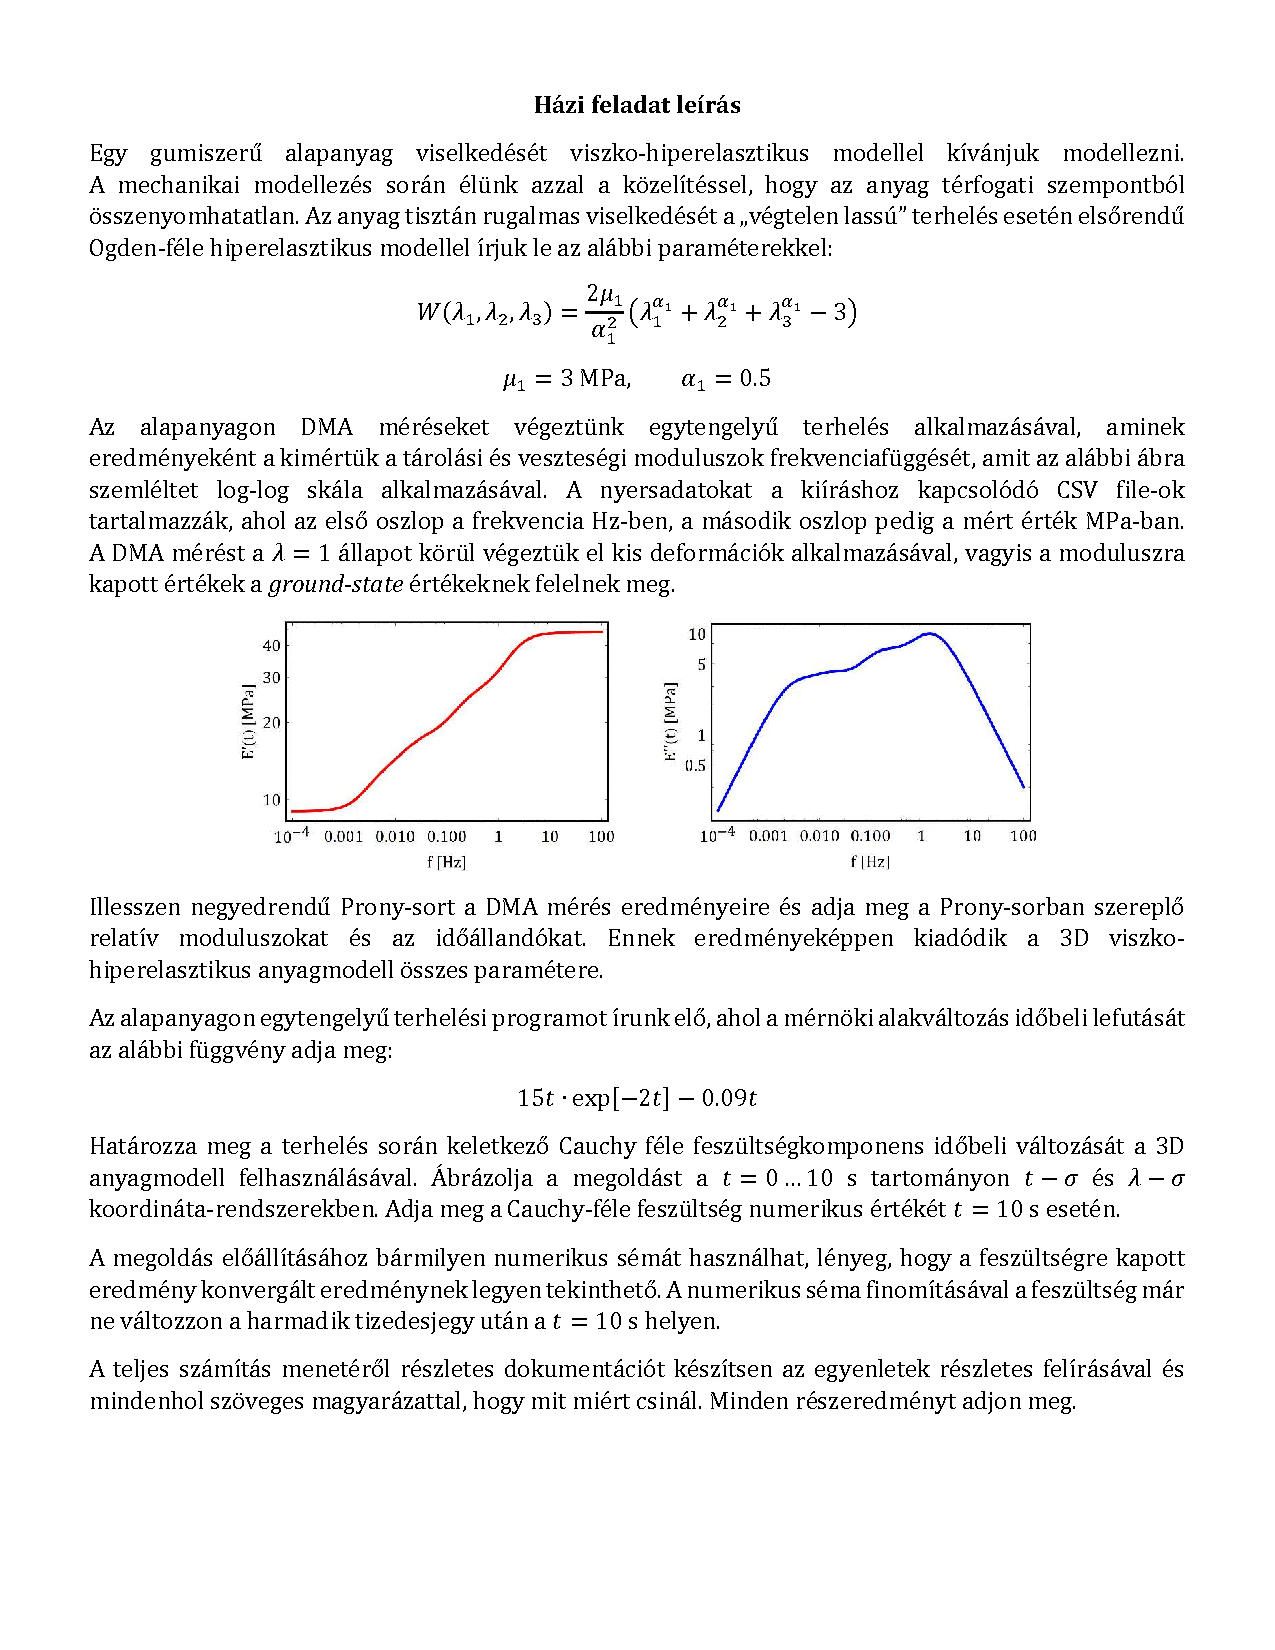
\includepdf[pages=-]{HF.pdf}
\newpage

\section{Determination of the Prony parameters}

The Prony parameters are used to describe the viscous behavior of materials. We can determine them by fitting the viscoplastic model's solution to the DMA experiment data. The measured quantities is the storage modulus $E'$ and the loss modulus $E''$, as shown in the Figure \ref{fig:experiment}.


\begin{figure}[h]
    \centering
    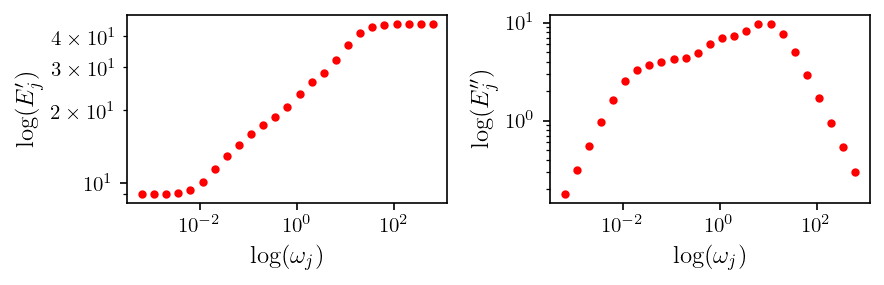
\includegraphics[scale=1]{figures/data.png}
    \caption{Virtual DMA experiment data}
    \label{fig:experiment}
\end{figure}

If relaxation modulus is expressed with an $N$th order Prony-series, the storage modulus $E'$ and the loss modulus $E''$ can be expressed as a function of the frequency $\omega$ as

\begin{equation}
E'(\omega) = 
E_{\infty} + \sum_{i=1}^N \frac{\tau_i^2 \omega^2}{1+\tau_i^2 \omega^2}E_i,
\end{equation}

\begin{equation}
E''(\omega) = 
\sum_{i=1}^N \frac{\tau_i \omega}{1+\tau_i^2 \omega^2}E_i,
\end{equation}

where the $E_{\infty},\{E_i\}_{i=1}^N$ and $\{\tau_i\}_{i=1}^N$ are the unknown Prony parameters. We will fit these functions on the measurement data, by optimizing the following objective function:

\begin{equation}
    Q\left(E_{\infty},\{E_i\}_{i=1}^N,\{\tau_i\}_{i=1}^N\right) = 
\frac{1}{n}\sum_{j=1}^n \left[\left(1-\frac{E'(\omega_j)}{E'_j}\right)^2 + \left(1-\frac{E''(\omega_j)}{E''_j}\right)^2\right].
\end{equation}

I used the \texttt{scipy.optimize.minimize} method for this purpose:  

\lstset{style=python}
\begin{lstlisting}
# order of the Prony series
N = 9 

# Initialize Prony parameters
E_inf = E_storage_true[0]
E = [E_inf/2] * N
tau = [1] * N

# Concatenate
initial_guess = [E_inf] + E + tau

# Define the bounds
bounds = [(0, None)] * len(initial_guess)

# Optimize
result = minimize(Q, initial_guess, bounds=bounds)
\end{lstlisting}

\newpage

We can repeat the optimization for different orders of the Prony series. On Figure \ref{fig:prony_order}. we can see how the final value of the objective function depends on the order of the choosen order of the Prony series.

\begin{figure}[H]
    \centering
    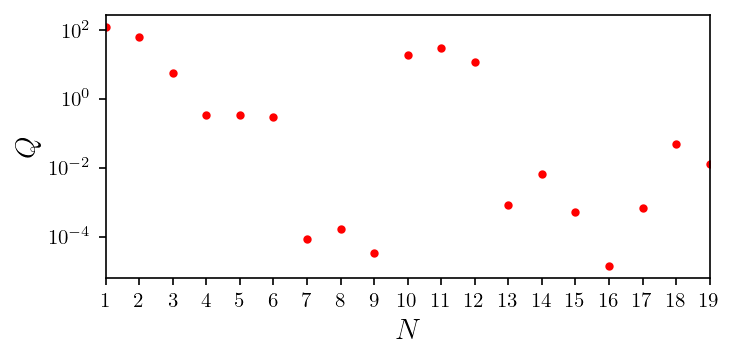
\includegraphics[scale=0.9]{figures/best_prony.png}
    \caption{The value of the objective function as a function of the order of the Prony series}
    \label{fig:prony_order}
\end{figure}

We can observe that the 16th and the 9th order Prony series gives the best fit. The 16th order is a bit better, but it is not worth to use such a high order, so we will use the 9th order one. The fitted 9th order Prony parameters are summarized in  Table \ref{tab:prony_parameters}.

\begin{table}[H]
    \centering
    \caption{Fitted Prony Parameters}
    \label{tab:prony_parameters}
    \begin{tabular}{|c|c|c|}
        \hline
        \textbf{i} & \textbf{Value of $E_i$} & \textbf{Value of $\tau_i$} \\ \hline
        $\infty$       & 8.9998                 & --                         \\ \hline
        $1$              & 0.9049                 & 49.7626                    \\ \hline
        $2$              & 0.9049                 & 49.7627                    \\ \hline
        $3$              & 0.9066                 & 49.7630                    \\ \hline
        $4$              & 0.9065                 & 49.7630                    \\ \hline
        $5$              & 0.9053                 & 49.7666                    \\ \hline
        $6$              & 9.0034                 & 0.9977                     \\ \hline
        $7$              & 17.9962                & 0.1000                     \\ \hline
        $8$              & 4.4825                 & 9.9175                     \\ \hline
        $9$              & 4.5023                 & 1.0000                     \\ \hline
    \end{tabular}
\end{table}

We can also plot the fitted storage and loss moduli against the measured data. The fitted curves are shown in Figure \ref{fig:fittedmodel}.
\begin{figure}[H]
    \centering
    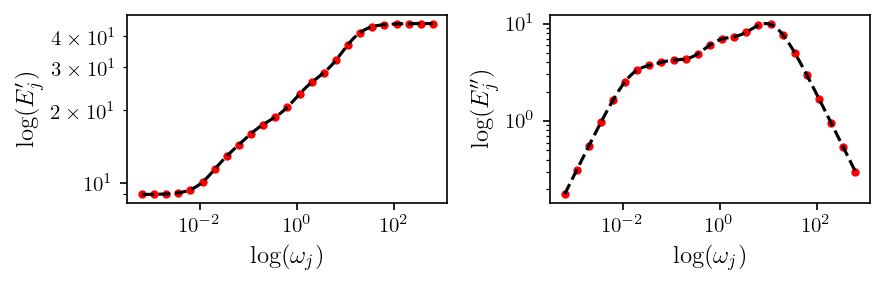
\includegraphics[scale=1]{figures/fitted.png}
    \caption{Fitted storage and loss moduli}
    \label{fig:fittedmodel}
\end{figure}

\newpage

From the Prony parameters we can determine the $E_0$ instantaneous modulus as

\begin{equation}
    E_0 = E_{\infty} + \sum_{i=1}^N E_i,
\end{equation}

from which we can determine the relative moduli as
\begin{equation}
    \{e_i\}_{i=1}^N = \left\{\frac{E_i}{E_0}\right\}_{i=1}^N.
\end{equation}

We have an incpomressible material, so the deviatoric part of the stress determines the volumetric part, therefore will assume that the relaxation characteristic defined by the previously calculated Prony parameters, belongs to the deviatoric behaviour, which means

\begin{equation}
    \{g_i\}_{i=1}^N = \{e_i\}_{i=1}^N.
\end{equation}

\section{The instantaneous stress response}

The purely elastic behavior of the material (under 'infinitely slow' loading) is described using a first-order Ogden-type hyperelastic model, which can be expressed as 

\begin{equation}
    W(\lambda_1, \lambda_2, \lambda_3) = \frac{2\mu_1}{\alpha_1^2} \left( \lambda_1^{\alpha_1} + \lambda_2^{\alpha_1} + \lambda_3^{\alpha_1} - 3 \right).
\end{equation}

We know that uniaxial loading is prescirbed. The solution of this model for the uniaxial loading was shown at continuum mechanics lectures. The Cauchy stress solution can be expressed as

\begin{equation}
\sigma_0 = P_0\cdot\lambda = \frac{2\mu_k}{\alpha_k}(\lambda^{\alpha_k} - \lambda^{-\frac{\alpha_k}{2}}).
\end{equation}

The engineering strain time evolution is given as

\begin{equation}
\varepsilon(t) = 15t\cdot e^{-2t}-0.09t,
\end{equation}

Therefore, the uniaxial stretch can be expressed as

$$
\lambda(t) = \varepsilon(t) + 1 = 15t\cdot e^{-2t}-0.09t + 1
$$
Substituting into the Cauchy stress equation, we can obtain the time evolution of the Cauchy stress. The result is shown in Figure \ref{fig:instantaneous_stress}.
\begin{figure}[H]
    \centering
    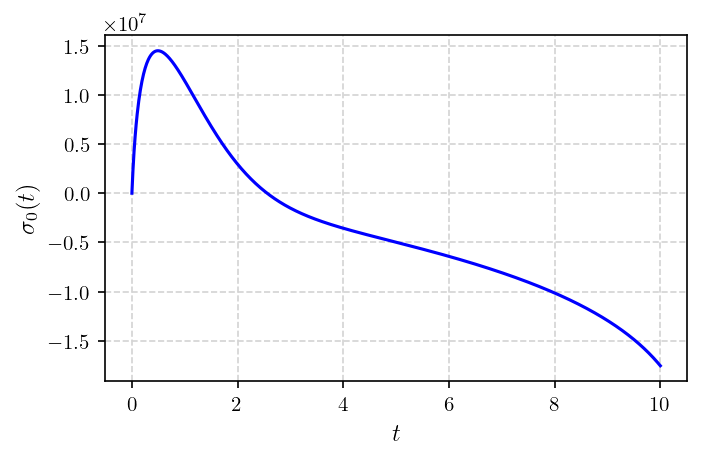
\includegraphics[scale=0.8]{figures/elastic_solution.png}
    \caption{Instantaneous stress response}
 \label{fig:instantaneous_stress}
\end{figure}

\newpage

\section{The viscoelastic stress response}

For uniaxial loading, the deviatoric part of the instantaneous Cauchy stress tensor can be expressed as

\begin{equation}
    \boldsymbol{s}_0(t) = 
    \sigma_0(t)
    \begin{bmatrix}
        2/3 & 0 & \\
        0 & -1/3 & 0\\
        0 & 0 & -1/3\\
    \end{bmatrix}
\end{equation}


We know from the lecture that, the deviatoric part of the stress can be expressed as

\begin{equation}
\boldsymbol{s}(t) = \boldsymbol{s}_0(t) - 
\text{dev}\left[
    \boldsymbol{F}(t)
        \left(
            \sum_{i=1}^N \frac{e_i}{\tau_i} \int_0^t \boldsymbol{F}^{-1}(t-s) \boldsymbol{s}_0(t-s) \boldsymbol{F}^{-T}(t-s)e^{-\frac{s}{\tau_i}}\text{d}s
        \right)
    \boldsymbol{F}^T(t)
\right].
\end{equation}

We know that the deformation gradient for uniaxial extension looks like

\begin{equation}
\boldsymbol{F}(t) = \boldsymbol{F}^T(t) = 
\begin{bmatrix}
    \lambda(t) & 0 & 0\\
    0&\lambda^{-1/2}(t)&0\\
    0&0&\lambda^{-1/2}(t)\\
\end{bmatrix},
\end{equation}

and it's inverse looks like

\begin{equation}
\boldsymbol{F}^{-1}(t) =  \boldsymbol{F}^{-T}(t)=
\begin{bmatrix}
    \lambda^{-1}(t) & 0 & 0\\
    0&\lambda^{1/2}(t)&0\\
    0&0&\lambda^{1/2}(t)\\
\end{bmatrix}.
\end{equation}

Everything is given to determine the deviatoric part of the stress. The only thing we need to do is to choose a numerical method to solve the convolutional integral. I used simple discrete convolution:

\lstset{style=python}
\begin{lstlisting}
# self defined convolution function
def conv(f,g,t):
    dt = t[1] - t[0]
    ret = [
        np.sum(f(t[k] - t[:k]) * g(t[:k]) * dt,axis=-1) 
        for k in range(len(t))
    ]
    return np.array(ret).T

# placeholder for the convolution result
SUM = np.zeros((3,len(t)))

# calculate the convolution terms
for i in range(len(tau)):
    f = lambda t: F_inv(t)*s0(t)*F_inv(t).T
    g = lambda t: np.e**(-t/tau[i])
    SUM += e[i]/tau[i] * conv(f,g,t)

# deviatoric stress
s = s0(t) - dev(F(t)*SUM*F(t).T)
\end{lstlisting}

\newpage

We can plot the deviatoric stress response as a function of time. The result is shown in Figure \ref{fig:viscoelastic_stress}.
\begin{figure}[H]
    \centering
    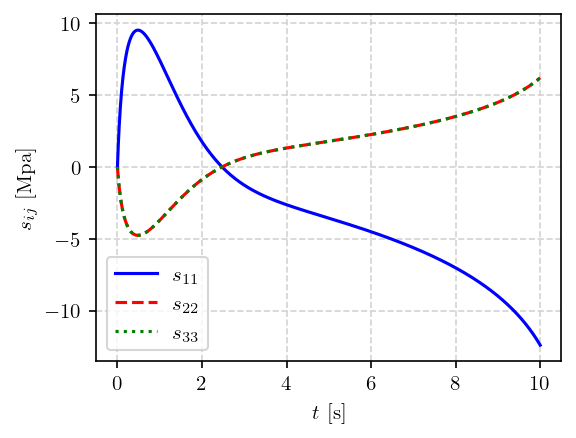
\includegraphics[scale=1]{figures/deviatoric_response.png}
    \caption{Deviatoric part of the stress response}
    \label{fig:viscoelastic_stress}
\end{figure}

The volumetric part of the stress can be calculated from the boundary conditions in the following way:

\begin{equation}
    \begin{matrix}
        \sigma_{22}(t) = s_{22}(t) + p(t) = 0, \\
        \sigma_{33}(t) = s_{33}(t) + p(t) = 0.
    \end{matrix}
\end{equation}

Therefore, we can express the volumetric part of the stress as
\begin{equation}
    \boldsymbol{p}(t) = - s_{22}(t)\boldsymbol{I}.
\end{equation}

The viscoelastic stress response can be expressed as

\begin{equation}
    \boldsymbol{\sigma}(t) = \boldsymbol{s}(t) + \boldsymbol{p}(t).
\end{equation}

We can be plot the result as the function of the time and the function of the strech. The result is shown in Figure \ref{fig:stress}.

\begin{figure}[H]
    \centering
    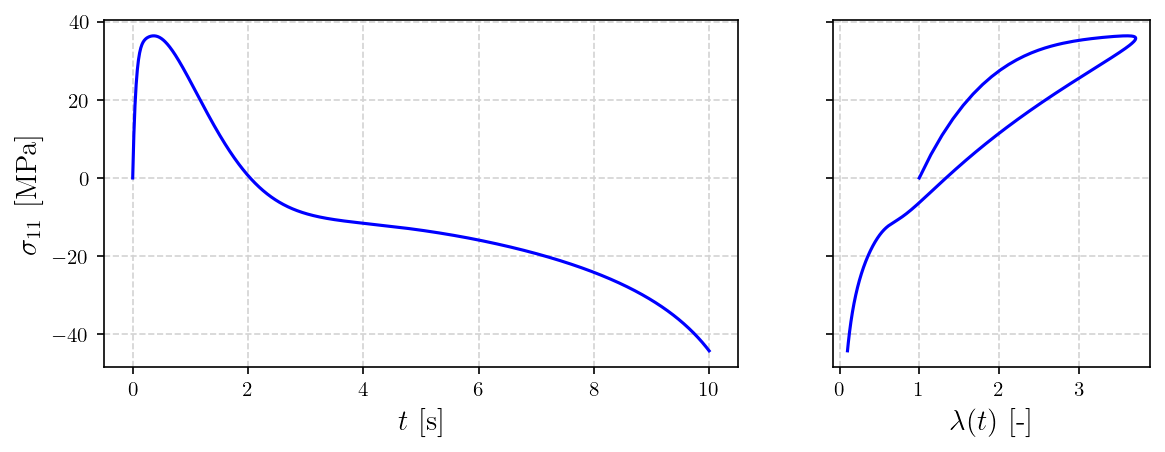
\includegraphics[scale=0.8]{figures/stress.png}
    \caption{Viscoelastic stress response}
    \label{fig:stress}
\end{figure}

\end{document}